\section{Evaluation Design}

This section defines the evaluation protocol used to compare architectural families while keeping educational claims, mechanism claims, and cost claims distinct. The paper now combines a forward-looking protocol with repository-grounded evidence, so the section serves two purposes: it explains how fair comparisons should be structured, and it clarifies how the current empirical snapshots should be interpreted.

\subsection{Comparison families and fairness principles}

The architectural families are operationalized as follows. \emph{Classical RAG} uses a single retrieve-then-generate pipeline with fixed retrieval access and no iterative planning loop. \emph{Agentic RAG} preserves retrieval but allows iterative planning, critique, rerouting, or tool use around the same grounding layer. \emph{Non-RAG multi-agent systems} rely on multiple specialized agents without a dedicated retrieval pipeline as the default controller. An optional \emph{single-agent no-RAG} baseline isolates retrieval and coordination effects from general model quality. Within agentic or multi-agent conditions, orchestration may be either always on or selectively invoked only for coordination-heavy or ambiguous tasks; we treat that as a configuration choice within the family rather than as a separate top-level family.

The comparison is built around architectural fairness, boundary-condition testing, and skeptical reading of output quality. The aim is not to produce one blended leaderboard, but to document where retrieval-heavy conditioning is decisive, where pedagogical coordination matters more, and where neither family earns a clean superiority claim. To keep cost arguments reproducible, each condition should report input and output tokens, cached-token usage when applicable, tool calls, planner or critic cycles, wall-clock latency, and estimated monetary cost per example or per dialogue.

\subsection{Task regimes and benchmark mapping}

Task regimes are separated explicitly so that retrieval-heavy and coordination-heavy workloads are not collapsed into a single aggregate score. Table~\ref{tab:task-regimes} summarizes the regimes, the kinds of learning activities they represent, and the architectural stresses they impose.

\begin{table}[t]
\centering
\small
\begingroup
\setlength{\tabcolsep}{4pt}
\begin{tabular}{@{}>{\raggedright\arraybackslash}p{0.26\linewidth}>{\raggedright\arraybackslash}p{0.32\linewidth}>{\raggedright\arraybackslash}p{0.17\linewidth}>{\raggedright\arraybackslash}p{0.2\linewidth}@{}}
\toprule
Regime & Representative learning activity & \shortstack[c]{Retrieval\\emphasis} & \shortstack[c]{Coordination\\emphasis} \\
\midrule
Evidence-grounded reasoning & Explain why the answer is correct with citations or reference material & High & Moderate \\
Rubric-based feedback & Provide diagnostic comments on student work using a rubric & Moderate & High \\
Adaptive tutoring & Diagnose misconceptions and offer next-step hints or mini-lessons & Low & High \\
Lesson/exercise planning & Produce sequences of learning activities aligned to goals & Low & Very high \\
\bottomrule
\end{tabular}
\endgroup
\caption{Task regimes that separate retrieval-heavy experiments from coordination-heavy ones.}
\label{tab:task-regimes}
\end{table}

The benchmark shortlist is filtered by three rules. Each candidate must map cleanly to one of these regimes, allow a contrast between at least two architectural families, and expose metrics or evaluation procedures that clarify \emph{why} an architecture performed better. Education-specific benchmarks such as EduBench, TutorEval, ScienceQA, MathTutorBench, and TutorBench support pedagogical claims \cite{xu2025edubench,chevalier2024sciencetutors,lu2022scienceqa,macina2025mathtutorbench,srinivasa2025tutorbench}. Transferable benchmarks such as HotpotQA, SCROLLS, LongBench v2, FEVER, Wizard of Wikipedia, BEIR, and AgentBench support narrower mechanism-level claims about retrieval depth, evidence justification, grounded dialogue, long-context handling, verification, and orchestration \cite{yang2018hotpotqa,shaham2022scrolls,bai2024longbench2,thorne2018fever,dinan2019wizard,thakur2021beir,liu2023agentbench}.

\begin{figure}[t]
\centering
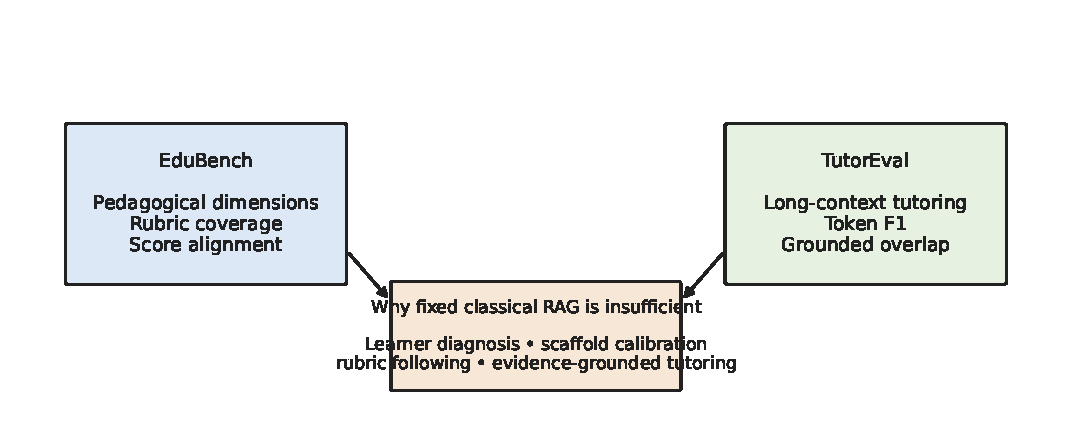
\includegraphics[width=0.92\linewidth]{build-artifacts/benchmark_metric_framing.pdf}
\caption{Benchmark and metric framing. Education-specific benchmarks justify pedagogical claims, while transferable benchmarks justify narrower mechanism-level claims.}
\label{fig:benchmark-framing}
\end{figure}

\begin{table*}[t]
\centering
\scriptsize
\begingroup
\setlength{\tabcolsep}{3.5pt}
\renewcommand{\arraystretch}{1.2}
\begin{tabular}{@{}>{\raggedright\arraybackslash}p{0.12\linewidth}>{\raggedright\arraybackslash}p{0.13\linewidth}>{\raggedright\arraybackslash}p{0.18\linewidth}>{\raggedright\arraybackslash}p{0.18\linewidth}>{\raggedright\arraybackslash}p{0.2\linewidth}>{\raggedright\arraybackslash}p{0.15\linewidth}@{}}
\toprule
Benchmark & Category & Main task family & Main metrics & Comparison utility & \shortstack[c]{Limitation for\\paper claims} \\
\midrule
EduBench & Education-specific & Multi-scenario educational QA, grading, and pedagogical support & Adaptation, accuracy, and pedagogy dimensions & Compares factual grounding with personalization and pedagogy & Evaluator-dependent; not a classroom-outcome benchmark \\
TutorEval / LM-Science-Tutor & Education-specific & Open-book vs. closed-book science tutoring QA & Key-point coverage and tutoring quality proxies & Contrasts retrieval-sensitive tutoring with explanation strategy & Domain-specific and evaluator-dependent \\
ScienceQA & Education-specific & Multimodal science QA with explanations and lecture context & Subject/context accuracy and explanation scoring & Probes explanation quality and grounded reasoning & Not a full tutoring-dialog benchmark \\
MathTutorBench / TutorBench & Education-specific & Tutoring dialogue with scaffolding or rubric-based feedback & Accuracy plus pedagogy/rubric metrics & Highlights coordination-heavy pedagogy & Subject- or rubric-specific \\
HotpotQA & Transferable & Multi-hop open-domain QA with supporting facts & Answer EM/F1 and supporting-fact metrics & Stresses retrieval depth and justification & Supports mechanism claims, not pedagogical claims \\
AgentBench & Transferable & Tool-using workflow completion and coordination & Task success rates across environments & Emphasizes coordination and tool-use stress testing & Not education-specific \\
SCROLLS / LongBench & Transferable & Long-context reasoning, QA, and summarization & Task-specific accuracy or ROUGE-style metrics & Stress test for long-context handling & Not pedagogy-specific \\
BEIR / FEVER / Wizard of Wikipedia & Transferable & Retrieval robustness, verification, and grounded dialogue & Retrieval and grounding metrics & Isolates retrieval quality before pedagogical claims & Supports retrieval-focused claims only \\
\bottomrule
\end{tabular}
\endgroup
\caption{Benchmark mapping for the evaluation protocol. Education-specific benchmarks support educational-usefulness claims, while transferable benchmarks support narrower mechanism-level claims.}
\label{tab:benchmark-map}
\end{table*}

\subsection{Metric families}

Evaluation combines automated metrics, human judgment, and cost reporting. The key design rule is separation: groundedness, pedagogical quality, adaptivity, robustness, and cost are reported independently so that no single blended score hides boundary conditions. Human raters should score outputs under architecture-blind conditions when feasible, using shared task-specific rubrics and a short calibration phase before full annotation. Where disagreement remains substantial, the protocol preserves that disagreement rather than forcing superficial consensus.

\begin{table}[t]
\centering
\small
\begin{tabular}{p{0.25\linewidth}p{0.6\linewidth}}
\toprule
Metric family & Reporting focus \\
\midrule
Groundedness & Citation recall/precision, hallucination counts, retrieval coverage, and alignment between retrieved snippets and claims. \\
Pedagogical quality & Human ratings for specificity, scaffolding, level alignment, clarity of next steps, and sensitivity to learner state. \\
Adaptivity & Evidence of maintaining student context, handling follow-up prompts, and adjusting to rubrics or learner models mid-dialogue. \\
Cost and latency & Token usage, tool calls, monetary cost, median latency, and p95 latency, along with any orchestration overhead. \\
Robustness & Failure-mode counts, rerun stability, and robustness to perturbations such as misspellings or conflicting goals. \\
\bottomrule
\end{tabular}
\caption{Metric families that keep groundedness, pedagogical quality, adaptivity, robustness, and cost separate.}
\label{tab:metric-families}
\end{table}

Keeping metric families separate does not prevent trade-off analysis. For deployment-oriented interpretation, the final study should analyze architectures under fixed latency budgets and under fixed quality thresholds. Under fixed latency, the question is which family yields stronger groundedness, pedagogical quality, and adaptivity. Under fixed quality thresholds, the question is how much time and cost each architecture requires to reach that level.

\subsection{Ablations and reviewer-facing controls}

The protocol anticipates several predictable objections. One ablation disables coordination layers inside agentic RAG to test whether retrieval alone explains its gains. Another adds retrieval to the strongest non-RAG multi-agent baseline to show whether grounding can rescue coordination failures. A third reduces tool-call or runtime budgets to confirm that reported wins are not artifacts of unbounded orchestration. The design also separates same-backbone comparisons from best-fit deployment comparisons: the former isolate architecture, while the latter answer the practical question of what a deployer should actually choose.

These controls matter because mixed or negative outcomes are informative. If classical RAG remains best on evidence-heavy tasks, that strengthens the taxonomy. If agentic or non-RAG coordination wins only when paired with substantially stronger or less deployable models, that becomes a boundary condition rather than a pure orchestration gain. The article therefore treats architecture choice as a context-sensitive systems decision, not as a one-direction replacement story.
